\documentclass[12pt,a4paper]{article}
\usepackage[utf8]{inputenc}
\usepackage[T2A]{fontenc}
\usepackage{amsmath,amssymb,amsfonts,amsthm}
\usepackage{graphicx}
\usepackage{xcolor}                 % Colors. Usage: \color{red} Red text
\usepackage{hyperref}               % Insert URL for external resource in the internet
\usepackage{cmap}                   % Search in PDF
\usepackage{mathtext}
\usepackage{icomma}                 % Smart comma
\usepackage{extsizes}
% Easy way to setup page paddings
\usepackage{geometry}
\geometry{top=25mm}
\geometry{bottom=35mm}
\geometry{left=35mm}
\geometry{right=20mm}
% Extra work with tables
\usepackage{longtable}  % Long tables
\usepackage{multirow}   % Several rows
\usepackage{multicol}   % Several columns
\usepackage{setspace} % Interline distance
\onehalfspacing % x1.5
%\doublespacing % x2
%\singlespacing % x1
% Highlighting
\usepackage{soul}
\usepackage{url}                % Lets you typeset urls.
% Setup hyperlighting
\usepackage{hyperref}
\hypersetup{
 unicode    = true,
 colorlinks = true,        % false: links in reactangles; true: color links
 linkcolor  = red,           % internal links within document
 citecolor  = green,         % link to bibliogrpahy
 filecolor  = magenta,       % link for files
 urlcolor   = cyan           % link to URLs
}

% Bibliogrpahy
\usepackage[backend=biber,bibencoding=utf8]{biblatex}
\addbibresource{references.bip}

% https://oeis.org/wiki/List_of_LaTeX_mathematical_symbols
\theoremstyle{plain}                
\newtheorem{theorem}{Theorem}[section]  
%======================================================================================
\title{\textbf{Parts of Deep Learning}}
\date{Last update: 9 MAY 2022}
\author{Konstantin Burlachenko (burlachenkok@gmail.com)}
%======================================================================================

\newcommand\sh[1]{\ensuremath{\mathop{\text{\normalfont ш}}#1}}

\begin{document}

\maketitle
\tableofcontents
\section{Introduction}
This document is a draft which I have created for purpose to systematize used tricks in various application around deep learning models. The all original papers are driven firstly by practice. This is not a note about that principle and it's pros. and cons. For some areas it's probably fine, for some does not.

\section{AlexNet}

The AlexNet paper "ImageNet Classification with Deep Convolutional Neural Networks" \cite{krizhevsky2012imagenet} is arguably the paper that brought deep learning to the forefront. After reading the paper \cite{krizhevsky2012imagenet} we can obtain the following main ten ideas from it.

\paragraph{First idea} Authors faced with situation that before them people work with smaller tasks and people provides in common the following suggestion in the area of computer vision:  \textit{"\dots collect larger datasets, learn more powerful models, and use better techniques for preventing overfitting\dots”}. For example before AlexNet was a work of LeCun, 1998 \cite{lecun1998gradient} and model with LeNet-5 which uses \textit{60K parameters}. Authors tried go beyond that.

\paragraph{Second idea} Architecture presented at \cite{krizhevsky2012imagenet}, Fig.1 carefully transform original input image. With several steps spatial dimension is reduced with 1 strided convolution (stride 4), and 3 max-pools. From another side channel dimension is increasing. The work empirically try to loose information very carefully. Finally input image is converted into long 4096 vector. During inference images are projected into that space. Finally there is a softmax into 1000 classes. What has been observed practically the importance of the depth of the network (in terms number of layers) which seems matters for vision tasks.

\paragraph{Third Idea} Authors have made the hugest up to date (at moment of 2012) model with \textbf{60 million parameters} to train a models with using 1.2 millions samples. In fact 1.2 million samples is still nothing for huge dimensional models. And due to that image classification task is not so easy due to a that inherited difficulty.
 
\paragraph{Fourth idea} Authors use Relu activation function, also known as $max(0,x)$ or $x_{+}$ for people from Optimization community. Original motivation of the authors was that it was practically impossible to train with sigmoid in that time, due to practically observing slower training time in case of using sigmoid activation function.

\paragraph{Fifth idea} Authors split layers across several GPUs by hands. And there is an additional trick as authors said the inter-GPU communication happened in a specific layers.

\paragraph{Sixth idea} Local Response Layer (LRL) try to “normalize” along channel (i.e. in each specific location for each feature map). Authors stated that for the task it appends generalization ability. Inspiration for this author obtained from research how real neurons behave.

\paragraph{Seventh idea} This paper make huge impact and momentum into Deep Learning technics modeling approach for tackle image classification tasks.

\paragraph{Eight idea} Network is trained on RAW RGB images with central crops which after uniform rescaling into 256 x H or W x 256 are cropped by central crop via obtaining 256x256. There is no use of SIFT or any specific Computer Vision algorithms for feature detection / important points detection.

\paragraph{Ninth idea} Data Augmentation generates artificially trained images on the fly. One extra thing authors found via PCA/SVD the need space for images and append unbiased noise for new images via adding random variables in that space.

\paragraph{Tenth idea} Use CNN layers for architecture by itself and build computation graph with that primitives. Use \textit{DropOut} regularization mechanism which in the same  time can reduce compute time and prevent over fitting. Where \textit{Dropout} is in fact a sampling mechanism across Neural Network architectures by itself.

\section{Example with arithmetic for counting filters}
Assume input image of size \textbf{55x55x3} and response or output of the convolution filter is \textbf{55x55x32}.

\paragraph{Number of filters}
Assume that by filter we use usual convolution which for depth tensor extension look completely into input channel.  We need under this assumption 32 filter, because output volume has 32 activation maps stacked together in the depth dimension/axis.

To go from input volume [55,55,3] given in HWC format to another volume [55,55,32] with filter size 5 and bias term we need 32 filters with spatial dimension [5,5] HW and zero padding occurs with in a format of SAME convolution.
Same convolution has padding such that $W_{out} = floor(W_{in} - F + 2P)/S + 1$ is the same as $W_{in}$.

\paragraph{Storage for all filter parameters}
The storage for this filter requires us $32x5x5x3$ parameters for convolution kernels and extra $32$ bias terms. And finally, we need $2432$ scalar parameters.

\paragraph{Storage for a single filter parameters}
For each filter, we need $5x5x3$ scalars describes filter and one single scalar for bias, a total of $76$ scalars for one filter.

\paragraph{Affect of strides and padding for number of parameters in a filter}
Stride convolution is a step with which filter with the rectangular or square form is sliding over the input tensor in both spatial dimensions. For classical convolution applied in CNN, there is the freedom to move in the depth dimension of input tensor for convolution kernel, because the kernel’s depth dimension is the same as the input dimension. Stride or Pad characteristics of convolution affect output tensor’s dimension in spatial extend (i.e. W and H) but the number of weights is the same for strided or not strided convolution.


...
Continue from Assignment 2.

\section{PointNet}
PointNet was introduced in work \cite{qi2017pointnet}. PointNet is working with geometry in the form of point clouds from $\mathbb{R}^3$. PointNet works with the set of unordered points. The motivation behind having PointNet building blocks is to have internal mechanisms that works with a set of points and which which are permutation invariant w.r.t. to the order of points in input specification.  Several operations are permutation invariant:
\begin{enumerate}
	\item Sharing weights for parallel implementation (per point) neural net is permutation invariant w.r.t. to order of input
	\item Max and Mean pooling are permutation invariant computation blocks w.r.t. to order of input
\end{enumerate}

This idea motivates  creates the following schema with several Multi Layer Perceptron(MLP) with weight sharing:

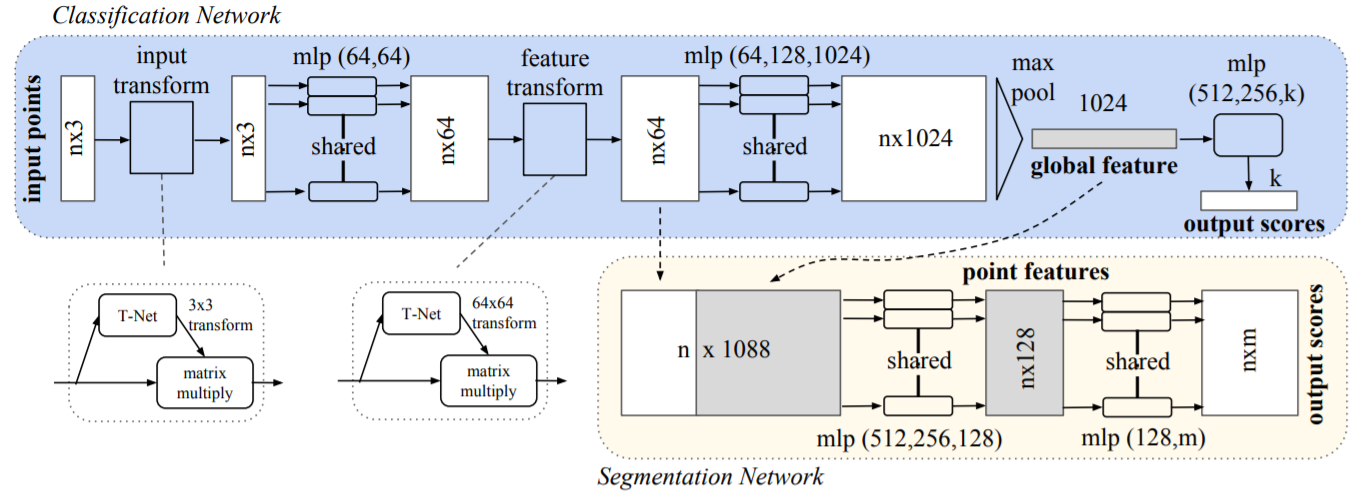
\includegraphics[width=\textwidth, keepaspectratio=true]{pointnet.png}

The near-final output is 128 feature vector per each point. PointNet achieved impressive performance on a few benchmarks, however:
\begin{enumerate}
	\item It cannot capture the local context on different scales
	\item No point in PointNet uses its local neighborhood, and it does not generalize well.
\end{enumerate}

\section{PointNet++}
PointNet++ has been introduced in a work \cite{qi2017pointnet++}. The main idea of PointNet++ is that it introduces a hierarchical neural network that applies PointNet recursively on a nested partitioning of the input point set. The hierarchical structure is composed of a number of set abstraction levels. There are three main features of PointNet:
\begin{enumerate}
	\item Usage of a Set Abstraction Level
	\item Multi-scale grouping to help with solving the problem with non-uniform density. This is achieved with features at different scales are concatenated to form a multi-scale feature and with random input dropout.
	\item In a set segmentation task such as semantic point labeling, we want to obtain point features for all the original points. The authors have appended a feature propagation mechanism to support that.
\end{enumerate}

The limitation of PointNet++:
\begin{enumerate}
	\item It works with points and ignores points relationship even if they exist
	\item It works with static points
	\item It does not support missing points or points with missing with one of the components
	\item Another inherited limitation of MLP. For example, the authors state that MLP is a universal continuous function approximation, and it's only partially true. More precisely, it's true only if have no limit to train data, and have the ability to infinitely blow up hidden layer. Both requirements are not valid in typical applications of Neural Nets. In case limit number of train set or limit topology MLP are not general function approximation.
\end{enumerate}

One of the most important components is a set abstraction level, and it is made of three key layers:
\begin{enumerate}
	\item \textbf{Sampling layer}. The Sampling layer selects a set of points from input points, which defines the centroids of local regions. We can call it anchors.
	\item \textbf{Grouping layer}. The grouping layer then constructs local region sets by finding "neighboring" points around the centroids.
	\item \textbf{PointNet layer}. The PointNet layer uses a mini-PointNet to encode local region patterns into a feature vector. PointNet is applied for the neighborhood to mimic convolution.
\end{enumerate}

The benefits of this layer:
\begin{enumerate}
	\item Learns "kernels" in compact space
	\item Kernels have compact spatial support similar to convolution with small compact support
	\item Suggest a concrete strategy to find central points for operations like convolution.
	\item It uses ideas like Inception with multi-scale
	\item It contains ideas similar to Drop-Out from CNN's
\end{enumerate}

\end{document}
